%% Beispiel-Präsentation mit LaTeX Beamer im KIT-Design
%% entsprechend den Gestaltungsrichtlinien vom Februar 2025
%%
%% Siehe https://sdq.kastel.kit.edu/wiki/Dokumentvorlagen

%% Beispiel-Präsentation
\documentclass{sdqbeamer}[en]
 
%% Gruppenlogo, muss im Verzeichnis logos/ liegen
%% falls kein Gruppenlogo gewünscht, bitte \grouplogo{} aufrufen
\grouplogo{codex_logo} 

%% Gruppenname und Breite (Standard: 89 mm)
\groupname{ITEC - Institute of Computer Engineering}
%\groupnamewidth{89mm}

% Beginn der Präsentation

\title[Design]{CodeX: Natural Language to Structured Code Generation}
\subtitle{Design} 
\author[Simon Bumiller]{Oleksandr Brittner, \textbf{Simon Bumiller}, Simon Gaber, Dayana Karadzhova, Kyrylo Pavlov \newline}

\date[23.\,1.\,2026]{January 23, 2026}

% Literatur 
 
%\usepackage[citestyle=authoryear,bibstyle=numeric,hyperref,backend=biber]{biblatex}
%\addbibresource{presentation.bib}
%\bibhang1em

\usepackage{lipsum}

\usepackage{pdfpages}

\begin{document}

%Titelseite
%\begin{frame}[title white vertical, picture=images/palladio_bauplan]
%	\titlepage
%\end{frame}

%\begin{frame}[title blue vertical, picture=images/palladio_bauplan]
%	\titlepage
%\end{frame}

\begin{frame}[title green horizontal, picture=images/circuit, kitlogo=white]
\titlepage
\end{frame}

%\begin{frame}[title white horizontal, picture=images/palladio_bauplan, kitlogo=white]
%\titlepage
%\end{frame}

%Inhaltsverzeichnis
\begin{frame}[tableofcontents=green]{Content}
	\tableofcontents
\end{frame}

%\begin{frame}[tableofcontents=blue]{Inhaltsverzeichnis}
%	\tableofcontents
%\end{frame}

\section{Intro}

\begin{frame}[t]{Introduction}{High-Level Architecture}

\begin{figure}
    \centering
    \begin{overprint}
        \onslide<1>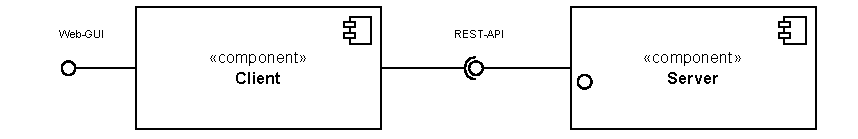
\includegraphics[width=27cm]{images/high-level}
        \onslide<2>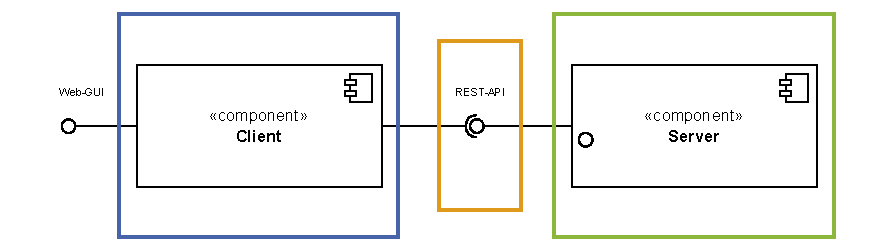
\includegraphics[width=27cm]{images/high-level-color}
    \end{overprint}
    \label{fig:placeholder}
\end{figure}

\begin{itemize}
    \item<2-> \textbf{\textcolor{kit-orange100}{System-Wide:}} Applies to the whole system
    \item<2-> \textbf{\textcolor{kit-blue100}{Client:}} Applies to the Client
    \item<2-> \textbf{\textcolor{kit-lightgreen100}{Server:}} Applies to the Server
    \item<2-> \textbf{Environment: } Everything else
\end{itemize}
\end{frame}

\section{System-Wide}

\begin{frame}{Authentication}{JWT's and Refresh Tokens}
    \textbf{JWT}
    \begin{itemize}
        \item Stateless tokens created by the server
        \item Presented with every request by the client
        \item Validity guaranteed by cryptographic signing with a private key
        \item Short-lived, ~15 minutes
    \end{itemize}
    \vspace{0.5em}
    \only<2->{\textbf{Refresh-Token}}
    \begin{itemize}
        \item<2-> Tokens persisted by the server
        \item<2-> Used to get new JWT's without having the user enter credentials (happens in background)
        \item<2-> Validity guaranteed by 'uniqueness' of UUID's
        \item<2-> Long-lived, ~1 month
        \item<2-> Rotated
    \end{itemize}
\end{frame}

\begin{frame}{Authentication}{Rationale}
    \textbf{Why not sessions?}
    \begin{itemize}
        \item JWT's are stateless
        \item Sessions require database/in-memory-cache lookup
        \item $\rightarrow$ Performance and System Complexity
    \end{itemize}
    \vspace{0.5em}
    \only<2->{\textbf{Why not only JWT's?}}
    \begin{itemize}
        \item<2-> Long-lived JWT's can be stolen and misused
        \item<2-> Frequent credential-based login is bad UX
    \end{itemize}
\end{frame}

\begin{frame}{Authorization}
    \textbf{Role-based}
    \begin{itemize}
        \item Different logical auth-roles: \textit{anonymous}, \textit{unverified}, \textit{normal}, \textit{admin}
        \item Most endpoints are allowed only for specific groups
        \item Authorization is a simple boolean-decision
    \end{itemize}
    \vspace{0.5em}
    \only<2->{\textbf{Owner-based}}
    \begin{itemize}
        \item<2-> Some resources are only exposed to the owner
        \item<2-> E.g.: Profile Data, Messages, LLM Configurations
        \item<2-> Database lookup is necessary to verify relations
    \end{itemize}
\end{frame}

\begin{frame}{REST-API}
    \begin{itemize}
        \item Only interaction between Client and Server $\rightarrow$ must be well-defined, to allow parallel implementation
        \begin{itemize}
            \item Endpoints: Paths, Request Bodies, Response Bodies, Path Variables, Query Parameters
            \item Authentication: Headers
            \item Schemas: Realized as DT's
        \end{itemize}
        \item Defined using OpenAPI
    \end{itemize}

    \vspace{0.5em}

    \only<2->{\textbf{OpenAPI}}
    \begin{itemize}
        \item<2-> Standardized format to describe REST-API's
        \item<2-> YAML format, interactive visualization into HTML/PDF
        \item<2-> Code generation, mock servers, validation 
    \end{itemize}
\end{frame}

\begin{frame}[plain]
\begin{center}
    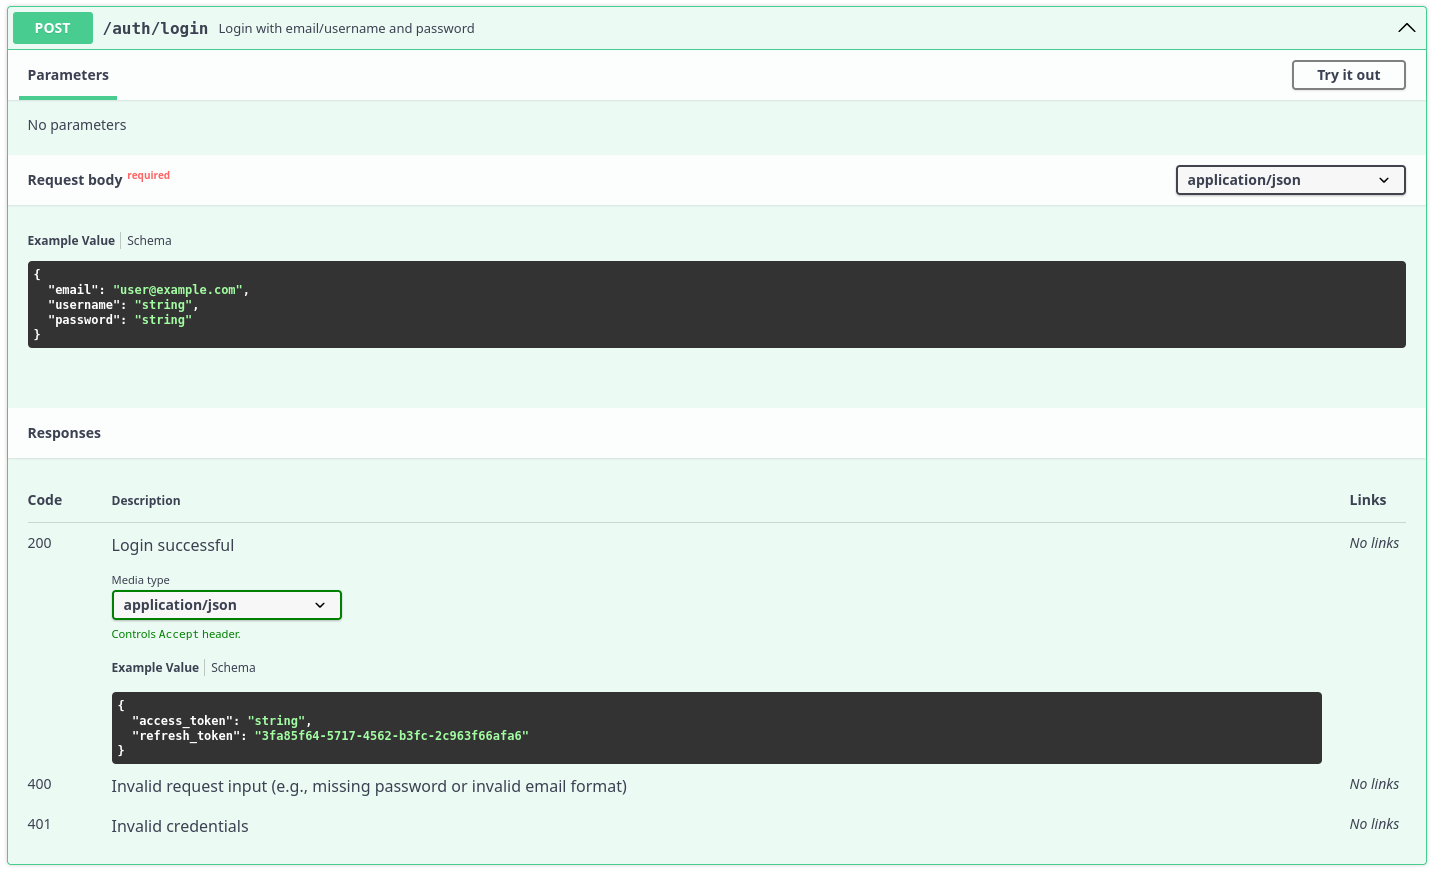
\includegraphics[height=\textheight]{images/openapi-example.png}
\end{center}
\end{frame}


\section{Client}

\begin{frame}{Client}{Overall Architecture}
\begin{columns}
    \column{\kitfourcolumns}
        \textbf{MVVM}
        \begin{itemize}
            \item Layered Architecture
            \item \textbf{View: } Display of Data, Interaction with user
            \item \textbf{ViewModel: } Source of State, handling user events
            \item \textbf{Model: } Source of Data, communication with external Services
        \end{itemize}
    \column{\kittwocolumns}
    \begin{figure}
    \centering
    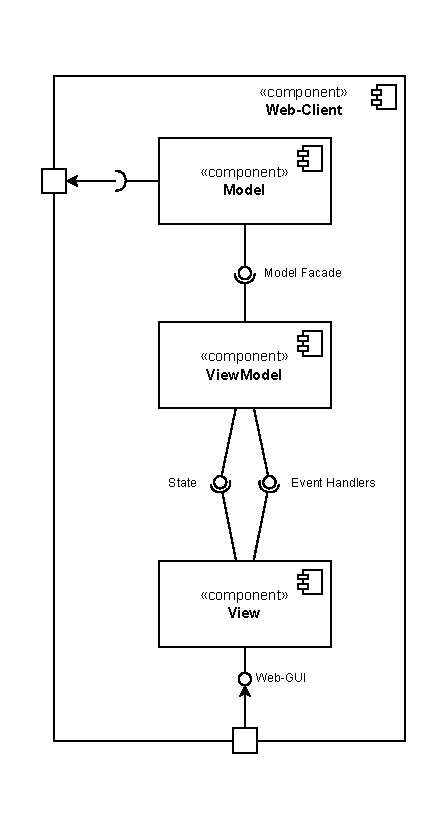
\includegraphics[height=11cm]{images/client}
    \label{fig:placeholder}
    \end{figure}
\end{columns}
\end{frame}

\begin{frame}{Client}{Model Architecture}
\begin{columns}
    \column{\kitfourcolumns}
        \textbf{Client Model}
        \begin{itemize}
            \item Data storage and communication with external services
            \item Distributed on submodules
            \item \textbf{Network: } Calling the \textit{REST-API}
            \item \textbf{Auhentication: } Handling refreshing of JWT's, current login status
            \item \textbf{Services: } Data caching and organization
        \end{itemize}
    \column{\kittwocolumns}
    \begin{figure}
    \centering
    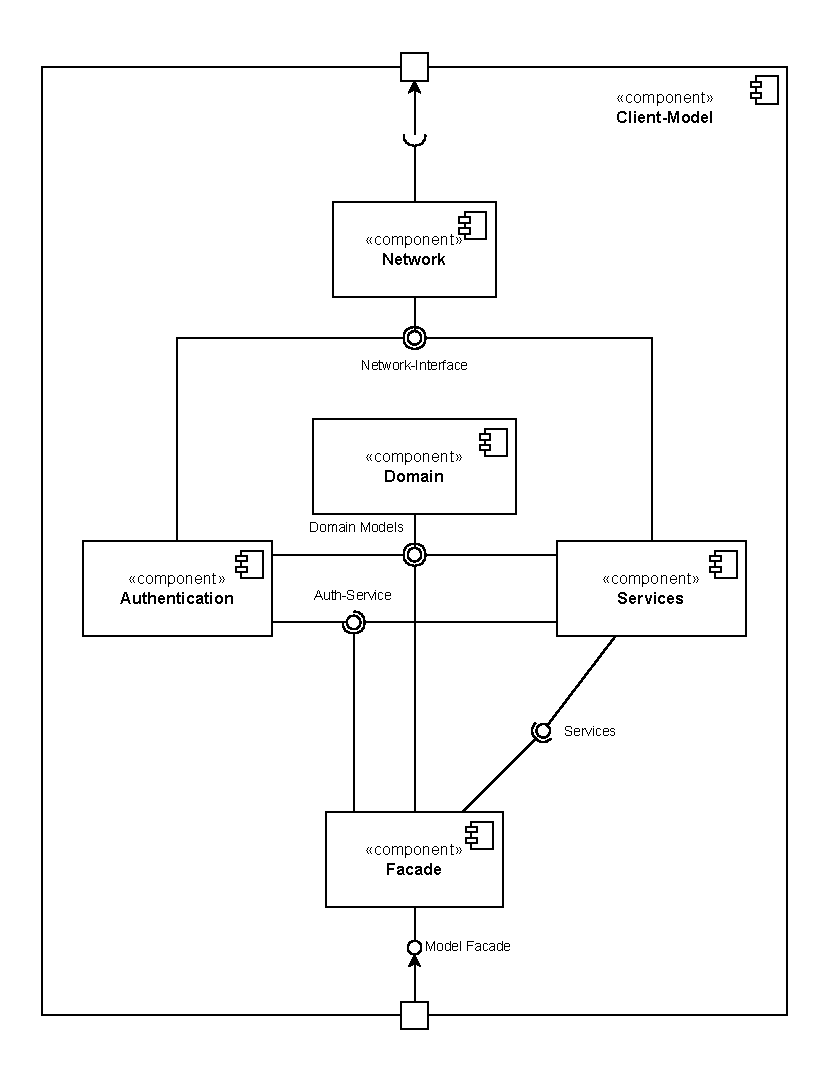
\includegraphics[height=11cm]{images/client-model}
    \label{fig:placeholder}
    \end{figure}
\end{columns}
\end{frame}

\begin{frame}{Client}{Rationale}
        \textbf{MVVM}
        \begin{itemize}
            \item \textit{View} and \textit{ViewModel} are automatically seperated when using \textbf{Angular}
            \item \textit{Model} is required to keep a local data cache
            \item \textit{Model} can be adapted to connect to a different datasource, while keeping interface
            \item \textit{Model} can be reused when the user interface changes. (e.g. angular web app $\rightarrow$ electron desktop app)
            \item All three components need drastically differing test-setups
        \end{itemize}
        
        \vspace{0.5em}
        
        \only<2->{\textbf{Seperation of concerns in Model}}
        \begin{itemize}
            \item<2-> Clear hierarchy: Network access is required for \textit{Authentication}
            \item<2-> \textit{Authentication} must be given when specific data is requested in \textit{Services}
        \end{itemize}

        \vspace{0.5em}

        \only<3->{\textbf{Angular and Typescript}}
        \begin{itemize}
            \item<3-> \textbf{Strong} and \textbf{static} typing system makes program structure clearer
            \item<3-> Component-based dependency-injection system makes source code closely related to component specification
            \item<3-> Default \textit{View-ViewModel} separation enforces structure (unlike e.g. react) 
        \end{itemize}
\end{frame}

\section{Server}

\begin{frame}{Server}{Architecture}
\begin{columns}
    \column{\kitfourcolumns}
        \textbf{Layered Architecture}
        \begin{itemize}
            \item Opaque Layered Architecture
            \item \textbf{Service: } Exposes the \textit{REST-API} to which clients will connect
            \item \textbf{Business: } Core logic: combines the single external services and implements functions specific to single user requests
            \item \textbf{Infrastructure and Persistence: } Connecting to the external services using their interfaces
        \end{itemize}
    \column{\kittwocolumns}
    \begin{figure}
    \centering
    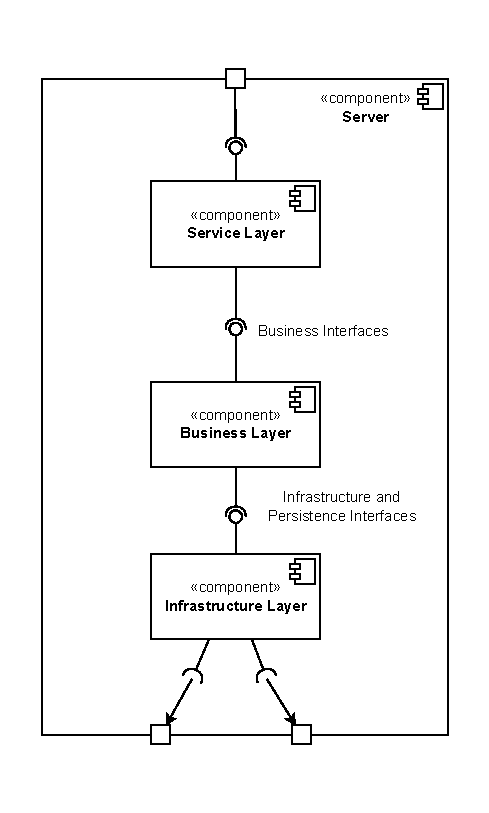
\includegraphics[height=11cm]{images/server}
    \label{fig:placeholder}
    \end{figure}
\end{columns}
\end{frame}

\begin{frame}{Server}{Rationale}
    \textbf{Abstraction over Infrastructure}
    \begin{itemize}
        \item Only \textit{Infrastructure Layer} knows about \textbf{how} the Database, Vector Database or LLM work
        \item Infrastructure can be exchanged (e.g. SQL $\rightarrow$ NoSQL) without adjusting \textit{Service} and \textit{Business}
    \end{itemize}

    \vspace{0.5em}

    \only<2->{\textbf{FastAPI and Python}}
    \begin{itemize}
        \item<2-> High development speed through simple syntax and gentle learning curve
        \item<2-> Tradeoff: Scalability, Structure and Security (alternative: Spring)
        \item<2-> Good integrations with \textit{SPICE} and LLM's
    \end{itemize}
\end{frame}

\section{Environment}

\begin{frame}{Database}
Detailed schema contained in appendix.
    \vspace{2em}
\break
    \textbf{Schema}
    \begin{itemize}
        \item \textbf{6 Tables: } \textit{Accounts}, \textit{Authentication Tokens}, \textit{Conversations}, \textit{Messages}, \textit{LLM Configurations}, \textit{Settings}
        \item \textbf{5 Relations} via foreign keys, \textbf{36} columns in total, \textbf{1} custom enum type
    \end{itemize}
    \vspace{0.5em}
    \only<2->{\textbf{Specific Design Decisions}}
    \begin{itemize}
        \item<2-> \textbf{UUID ID's: } Prevent \textit{ID enumeration} by using 'random' sequences
        \item<2-> \textbf{Auth-Token-Type enum instaed of seperate tables: } Rather differentiate the type of a token than duplicating table structures
    \end{itemize} 
\end{frame}

\begin{frame}{Deployment with Docker}
    \begin{itemize}
        \item \textbf{Docker: } Widely used technology, extensiond like Docker-Compose or Docker-Swarm 
        \item \textbf{Seperate Client and Server Container: } Easier testing, flexible scaling
        \item \textbf{Database and LLM as external services: } Integrates well with docker, decouples those versions from the system 
    \end{itemize}
\end{frame}

\begin{frame}{}
\vspace{4em}
\begin{center}
     \Large\textbf{\textcolor{kit-blue60}{Any further questions?}}
\end{center}
\end{frame}

\end{document}